\documentclass[twoside,twocolumn]{article}

\usepackage{blindtext} % Package to generate dummy text throughout this template 
\usepackage{graphicx}
\usepackage[sc]{mathpazo} % Use the Palatino font
\usepackage[T1]{fontenc} % Use 8-bit encoding that has 256 glyphs
\linespread{1.05} % Line spacing - Palatino needs more space between lines
\usepackage{microtype} % Slightly tweak font spacing for aesthetics

\usepackage[english]{babel} % Language hyphenation and typographical rules

\usepackage[hmarginratio=1:1,top=32mm,columnsep=20pt]{geometry} % Document margins
\usepackage[hang, small,labelfont=bf,up,textfont=it,up]{caption} % Custom captions under/above floats in tables or figures
\usepackage{booktabs} % Horizontal rules in tables

\usepackage{lettrine} % The lettrine is the first enlarged letter at the beginning of the text

\usepackage{enumitem} % Customized lists
\setlist[itemize]{noitemsep} % Make itemize lists more compact

\usepackage{abstract} % Allows abstract customization
\renewcommand{\abstractnamefont}{\normalfont\bfseries} % Set the "Abstract" text to bold
\renewcommand{\abstracttextfont}{\normalfont\small\itshape} % Set the abstract itself to small italic text

\usepackage{titlesec} % Allows customization of titles
\renewcommand\thesection{\Roman{section}} % Roman numerals for the sections
\renewcommand\thesubsection{\roman{subsection}} % roman numerals for subsections
\titleformat{\section}[block]{\large\scshape\centering}{\thesection.}{1em}{} % Change the look of the section titles
\titleformat{\subsection}[block]{\large}{\thesubsection.}{1em}{} % Change the look of the section titles

\usepackage{fancyhdr} % Headers and footers
\pagestyle{fancy} % All pages have headers and footers
\fancyhead{} % Blank out the default header
\fancyfoot{} % Blank out the default footer
\fancyhead[C]{El Aseguramiento de la Calidad de Software  $\bullet$ Mayo 2019 $\bullet$ } % Custom header text
\fancyfoot[RO,LE]{\thepage} % Custom footer text

\usepackage{titling} % Customizing the title section

\usepackage{hyperref} % For hyperlinks in the PDF

%----------------------------------------------------------------------------------------
%	TITLE SECTION
%----------------------------------------------------------------------------------------

\setlength{\droptitle}{-4\baselineskip} % Move the title up

\pretitle{\begin{center}\Huge\bfseries} % Article title formatting
\posttitle{\end{center}} % Article title closing formatting
\title{ Pentesting} % Article title
\author{
    Jorge Pacora Silva
    \and
    Adnner Esperilla
}
\date{\today} % Leave empty to omit a date
\renewcommand{\maketitlehookd}{%
\begin{abstract}
\noindent The purpose of this presentation is to provide an overview of the application of penetration
testing to secure systems administration. As such, the presentation is not overly technical in scope, but
covers instead what penetration testing is, what benefits stakeholders in a secure system receive from a
test, and how policies can aid or hinder penetration testing.
Penetration testing is a specialized security auditing method where a tester simulates an attack
on a secured system. The goal of this is not to cause damage, but instead to identify attack surfaces,
vulnerabilities, and other security weaknesses from the perspective of an attacker. Such testing can
range across all aspects of a system; the areas of computer, operational, personnel, and physical
security can all encompass potential weaknesses that a malicious attacker can exploit, and thus a
penetration tester may examine. Depending on the organization's priorities, risk assessment, and
policies, some of these areas may be out of scope or not deemed as important, so a reduced scope
penetration test may be conducted. 
\end{abstract}
}

%----------------------------------------------------------------------------------------

\begin{document}

% Print the title
\maketitle

%----------------------------------------------------------------------------------------
%	ARTICLE CONTENTS
%----------------------------------------------------------------------------------------

\section{Introduccion}

\lettrine[nindent=0em,lines=3]{P}odemos defenir que son normalmente un conjunto de “tests de penetración” basados en ataques hacia sistemas informáticos con la intencionalidad de encontrar debilidades y/o vulnerabilidades relativas a la seguridad, pudiendo clasificar más determinar el alcance y la repercusión de las mismas.

%------------------------------------------------
\section{TITULO}
\begin{itemize}
\item APLICACION DE PENTESTING
\end{itemize}
%------------------------------------------------
\section{AUTORES}
\begin{itemize}
\item Adnner Esperilla Ruiz
\item Pacora
\end{itemize}
%------------------------------------------------
\section{PLANTEAMIENTO DEL PROBLEMA}
\subsection{Problema}
\begin{itemize}
\item La Municipalidad de Pocollay, es una
entidad del estado, del orden territorial y a favor de la comunidad, cuyo objetivo es velar y
prestar sus servicios públicos con el cumplimiento de un rol fundamental para con la
población, ya que como institución pública, autónoma y jurídicamente hablando, puede
promover e implementar toda clase de actividades políticas, económicas, sociales y
culturales, con la visión de satisfacer las necesidades de la comunidad.\\
El ente territorial en su principio de actualización e inmersión tecnológica para todos y cada
uno de los procesos que se generan funcionalmente, ha implementado un sistema
distribuido de red de computadoras LAN (Local Área Network) la cual permite compartir
recursos Software, Hardware e información, elementos que deben contar con
confidencialidad, Integralidad y disponibilidad.\\
Dicha situación conlleva a una nefasta perdida, robo o destrucción de la información,
suplantación de identidad de funcionarios, virus informáticos, fallos en los sistemas de
información, mal funcionamiento del Hardware, intermitencia o caída de la red (offnet),
Spoffing de DNS, IP o DCHP, denegación del servicio (DoS), ingeniería social, entre otras
situaciones críticas que afectan el funcionamiento de una red y sus servicios.

\subsection{Justificacion}
\end{itemize}
El desarrollo de esta investigación le permitirá a la Municipio de Pocollay, contar con red de computadoras y sus respectivos servicios de forma segura,
permitiendo generar un alto grado de confidencialidad, Integralidad y disponibilidad de la
información.\\
Los análisis de vulnerabilidades o PenTesting permitirán determinar el nivel de seguridad
en: un equipo, en la red de equipos LAN (Local Área Network) o WLAN (Wireless local
Área Network), aplicaciones Web, Servidores de Información, entre otros, por medio de
ataques informáticos simulados idénticos a los que realizaría un Cracker o Black Hat
Hacker pero sin poner en riesgo la información o la disponibilidad de los servicios, esto se
hace con el fin de encontrar las posibles amenazas o vulnerabilidades en los sistemas
informáticos antes de que las descubra un atacante (externo o interno).
\subsection{Alcance}
\end{itemize}
El proyecto de investigación se desarrollará tomando como punto de partida los elementos
o fases de la investigación cualitativa. Determinando un alcance de procedimientos
exploratorios, y teniendo en cuenta los diferentes métodos y técnicas propias de cada una
de las etapas que se abordaran en el estudio, incluyendo los procedimientos, recolección,
procesamiento y análisis de la información, además del seguimiento al cronograma de
actividades.
\section{OBJETIVOS}
\subsection{General}
\end{itemize}
Describir los problemas de seguridad de la red de computadoras en Municipalidad de 
Pocollay, a través de pruebas de penetración que permitan el
mejoramiento continuo de la entidad
\subsection{Especificos}
\end{itemize}
\item Realizar un pentesting “prueba de penetración” para la determinar qué tipo de
vulnerabilidades presenta la red de computadoras en el Municipio de Pocollay
\item Identificar los diferentes ataques a los que está expuesta la red de computadoras y sus
servicios.
\item Generar recomendaciones que reduzcan la vulnerabilidad de la red de computadoras
\section{REFERENTES TEORICOS}
\item Disponibilidad: Hace referencia a la capacidad de un sistema que permite realizar consultas
en la medida que se requiera de una manera rápida y eficaz por el personal autorizado.
También se refiere a la capacidad de que la información pueda ser recuperada en el
momento que se necesite.
\item Confidencialidad: hace referencia a la privacidad de la información, la seguridad
informática debe proteger un sistema informático de acceso a la información por parte de
personal o programas no autorizados.
\item Integridad: Es la cualidad que posee un documento o archivo que no ha sido alterado y que
además permite comprobar que no se ha producido manipulación alguna en el documento
original.
\section{DESARROLLO DE LA PROPUESTA}
\subsection{Tecnologias de Informacion}
\end{itemize}
Las Herramientas a Utilizar para realizar esta propuesta de Desarrollo
son las siguientes :
\item Android Studio
\item ILenguaje Java , Xml
\item Sqlite
\item Nmap
\item Metasploit
\subsection{Metodología, técnicas usadas}
\end{itemize}
\item Metodologia Scrum
\section{FIGURAS}
\begin{center}
    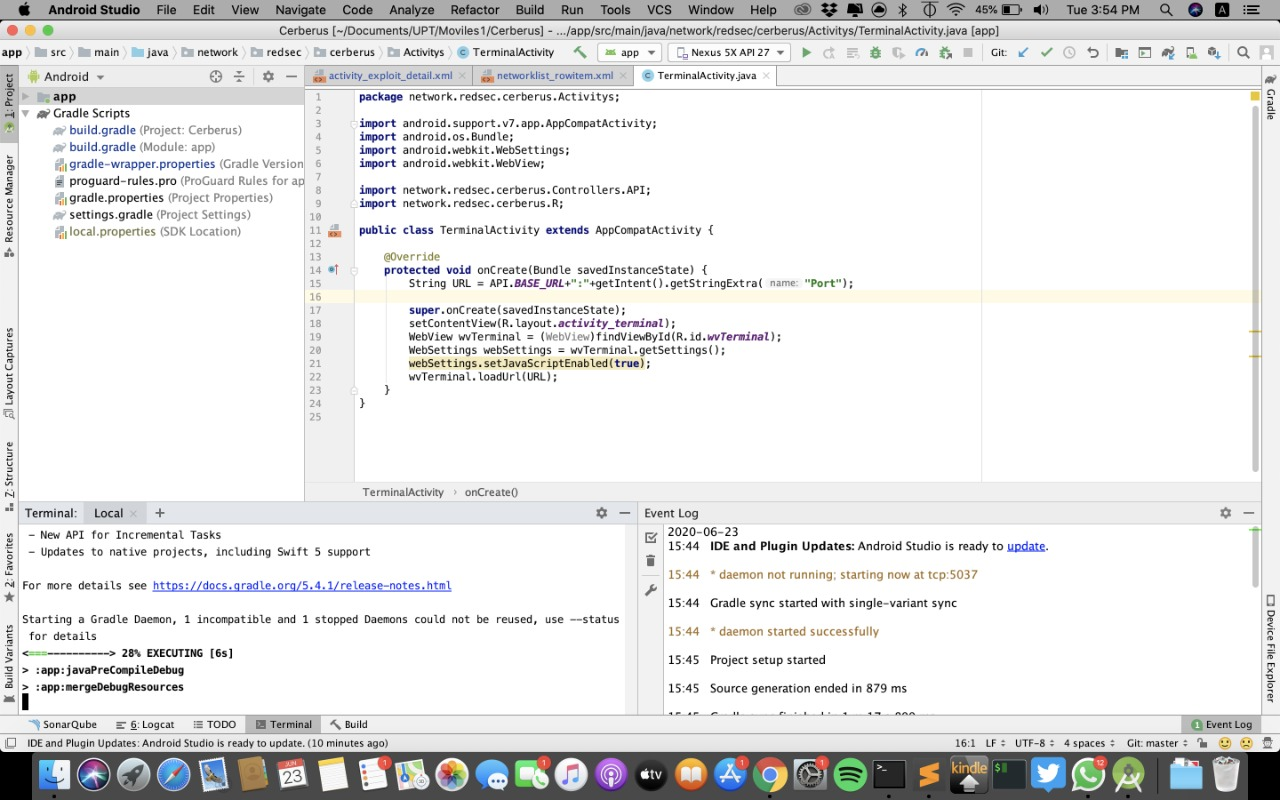
\includegraphics[width=8cm]{Pentesting/Imagenes/WhatsApp Image 2020-06-23 at 3.54.43 PM.jpeg}
    
    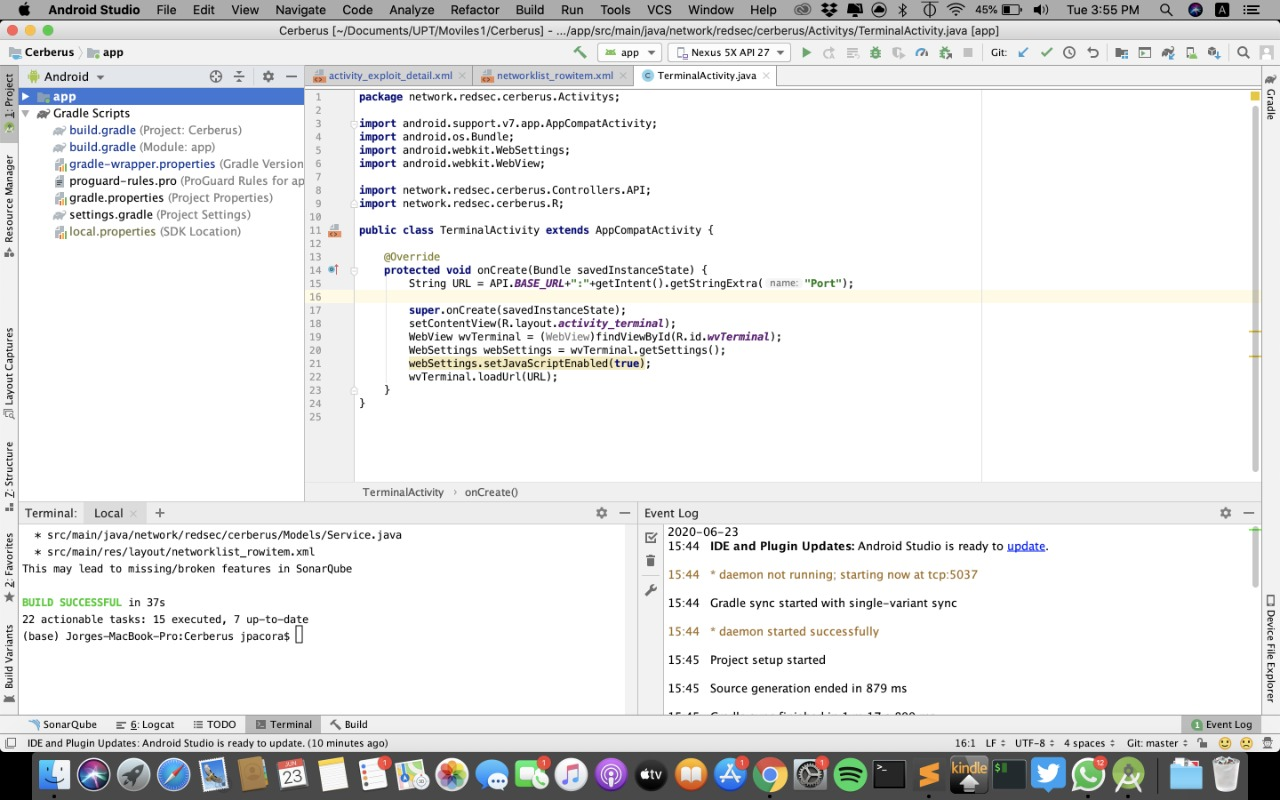
\includegraphics[width=8cm]{Pentesting/Imagenes/WhatsApp Image 2020-06-23 at 3.55.13 PM.jpeg}
    
    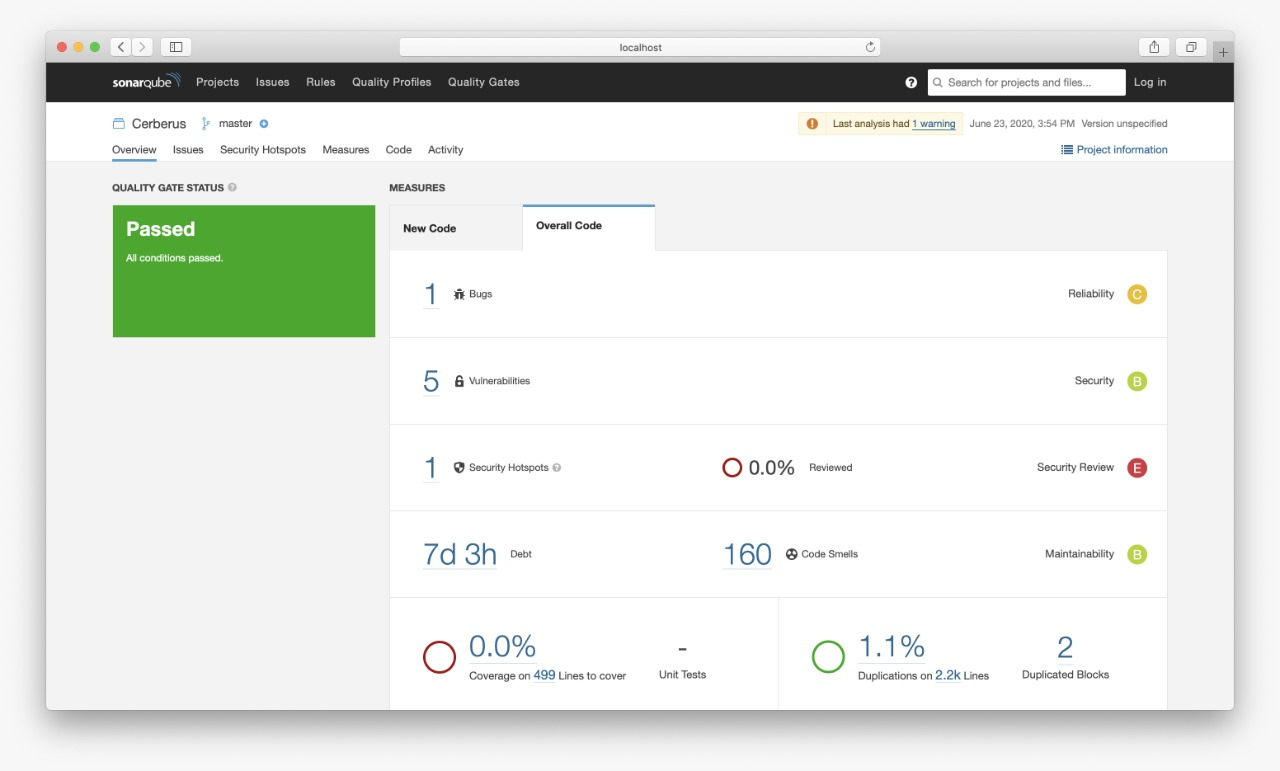
\includegraphics[width=8cm]{Pentesting/Imagenes/WhatsApp Image 2020-06-23 at 3.56.38 PM.jpeg}
    
    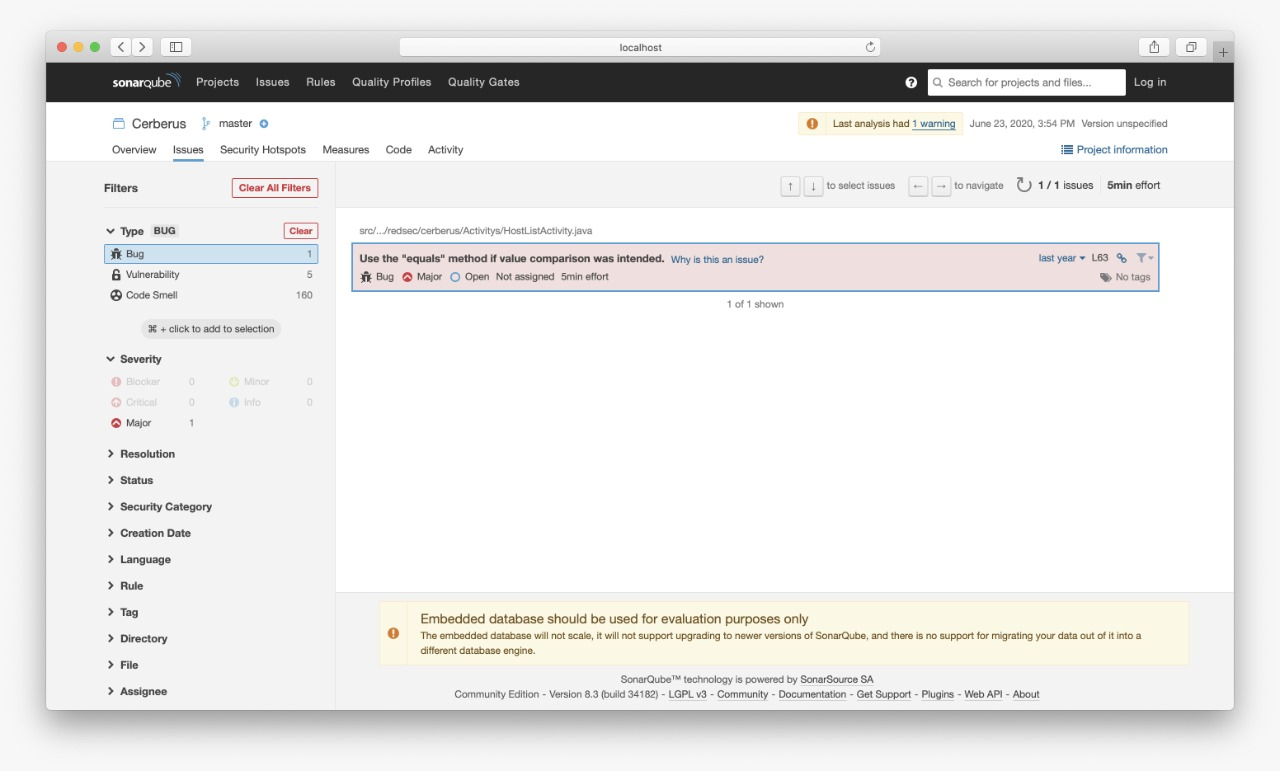
\includegraphics[width=8cm]{Pentesting/Imagenes/WhatsApp Image 2020-06-23 at 3.57.11 PM.jpeg}
    
    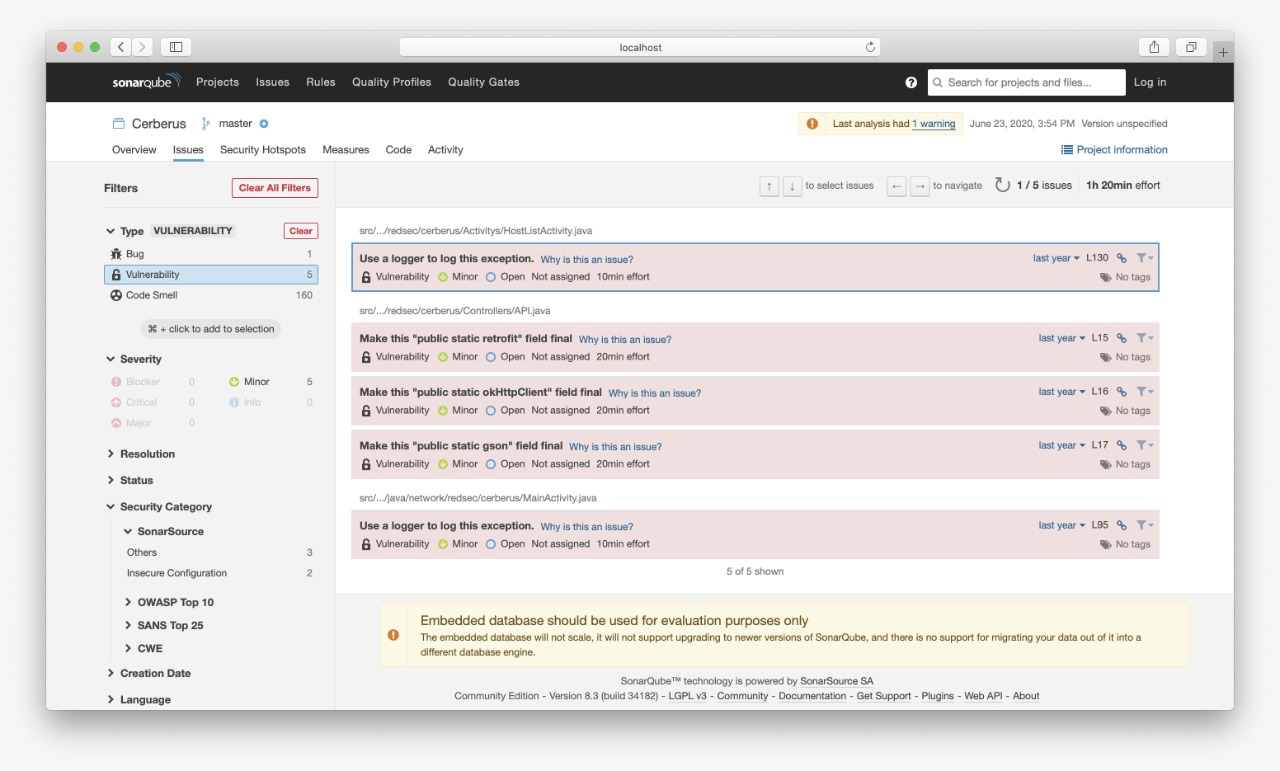
\includegraphics[width=8cm]{Pentesting/Imagenes/WhatsApp Image 2020-06-23 at 3.57.32 PM.jpeg}
    
    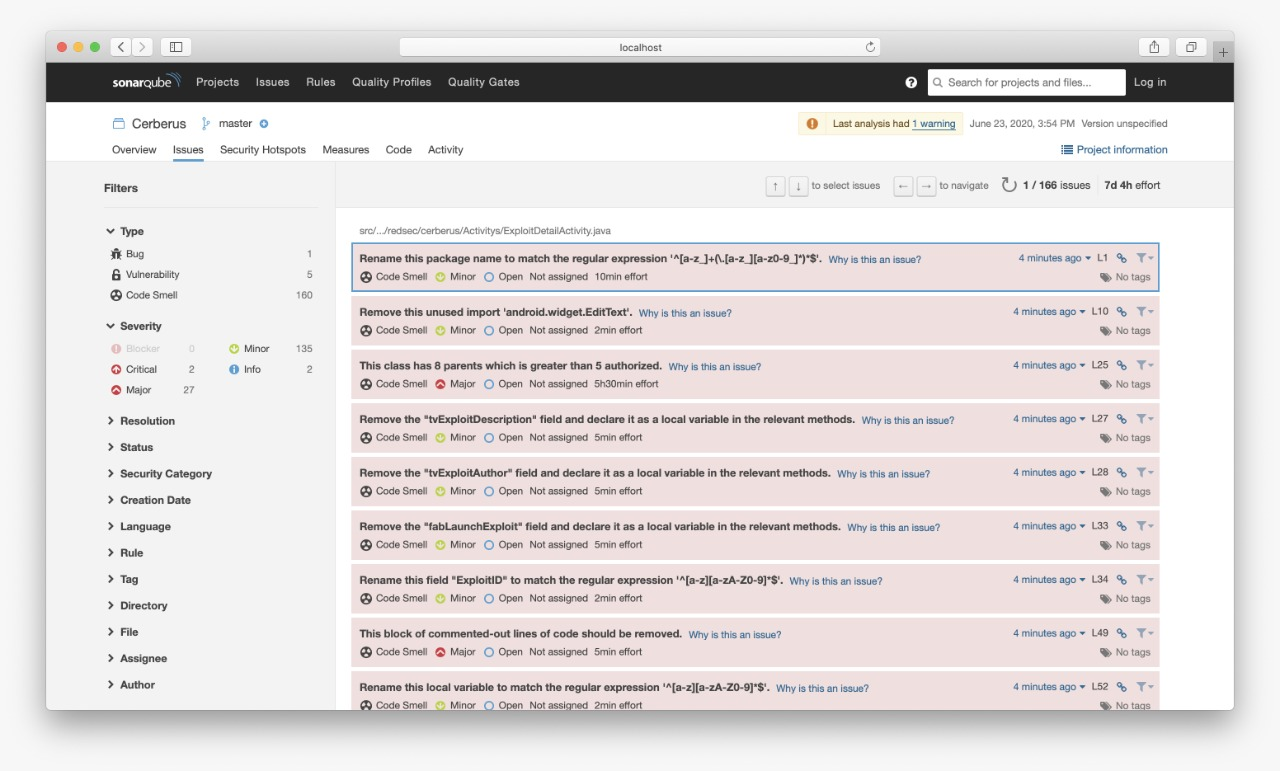
\includegraphics[width=8cm]{Pentesting/Imagenes/WhatsApp Image 2020-06-23 at 3.59.25 PM.jpeg}
    
    
\end{center}
\section{CRONOGRAMA}
\begin{center}


	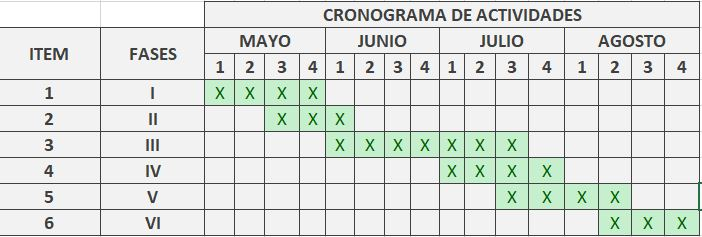
\includegraphics[width=8cm]{./Imagenes/CRONOGRAMA} 
	\end{center}
\item Fase I: Identificación de las diferentes fuentes de información que permitirán ampliar la
perspectiva del conocimiento a aplicar.
\item Fase II: Análisis y clasificación de la información según su género, origen y categoría. 
\item Fase III: Selección y aplicación de las herramientas de Pentesting “Prueba de Penetración”
para determinar las vulnerabilidades de la red de computadoras y sus servicios.
\item Fase IV: Análisis de resultados obtenidos de la red de computadores y sus servicios e
identificación de las vulnerabilidades
\item Fase V: Aplicación de medidas correctivas y sugerencias para mitigar las vulnerabilidades
de la red de computadora y sus servicios.
\item Fase VI: Conclusiones y elaboración de un Documento final.






\end{document}
